\resizebox{1\columnwidth}{!}{
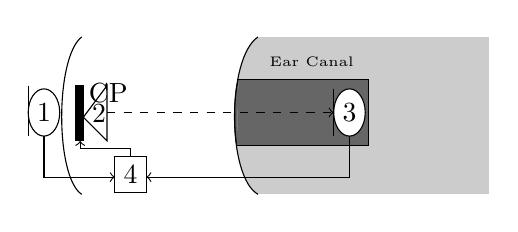
\begin{tikzpicture}
\draw [](-2.92,2.32) node (v1) {} .. controls (-3.26,2.06) and (-3.26,0.54) .. (-2.92,0.32) node (v2) {};

\draw [draw=black,fill=black!20](-0.68,2.32) node (v1) {} .. controls (-1.08,2.06) and (-1.08,0.54) .. (-0.68,0.32) node (v2) {};
\draw [white, fill=black!20](-0.68,2.32) -- (2.26,2.32) -- (2.26,0.32) -- (-0.68,0.32);


\draw [draw=black,fill=black!60](-0.93,1.78) node (v1) {} .. controls (-0.99,1.59) and (-0.99,1.14) .. (-0.95,0.94) node (v2) {};
\draw [draw=black,fill=black!60](-0.93,1.78) -- (0.72,1.78) -- (0.72,0.94) -- (-0.95,0.94);


\draw [draw=black,fill=white] (0.48,1.36) node (v3) {3} ellipse (0.2 and 0.3);
\draw [draw=black,fill=black](0.28,1.66) -- (0.28,1.06);

\draw [draw=black,fill=white] (-3.4,1.36) node (v3) {1} ellipse (0.2 and 0.3);
\draw [draw=black,fill=black](-3.6,1.7) -- (-3.6,1.06);


\draw [draw=black,fill=black] (-2.9,1.7) rectangle (-3,1);
\draw (-2.9,1.3) -- (-2.6,1.7) -- (-2.6,1) -- (-2.9,1.3);
\node at (-2.7,1.34) {2};


\draw[->,dashed] (-2.6,1.36) node[right=0.5,above]{CP}-- (0.28,1.36);
\draw  (-2.1,0.8) rectangle node{4}(-2.5,0.34);
\draw [<-](-2.5,0.54) -- (-3.4,0.54) -- (-3.4,1.06);
\draw [<-](-2.1,0.54) -- (0.48,0.54) -- (0.48,1.06);
\draw [->](-2.3,0.8) -- (-2.3,0.9) -- (-2.94,0.9) -- (-2.94,1);
\node at (0,2) {\tiny{Ear Canal}};
\end{tikzpicture}}